
%%*******************************************************************
%%  COBEP 2015 LateX Class
%%
%%  Version 2.0 
%%
%%  Last Modification - 17/09/2015
%%
%%  Copyright 2015 
%%
%%  This work may be distributed and/or modified under the
%%  conditions of the LaTeX Project Public License, either version 1.3
%%  of this license of (at your option) any later version.
%%  The latest version of this license is in
%%    http://www.latex-project.org/lppl.txt
%%  and version 1.3 or later is part of all distributions of LaTeX
%%  version 2005/12/01 or later.
%%
%%  The Current Maintainer of this work is Adriano Ruseler.
%%*******************************************************************

\documentclass[english]{cobep-spec}


%For all other papers the copyright notice is: “978-1-4799-8779-5/15/$31.00 ©2015 IEEE”.
\copyrightnotice{978-1-4799-8779-5/15/\$31.00 \copyright 2015 IEEE}

\title{ENGLISH GUIDELINES FOR PUBLICATION - TITLE HERE \\(14 PT TYPE SIZE, UPPERCASE, BOLD, CENTERED)}

\author{Adriano Ruseler$^{1}$, Telles Brunelli Lazzarin$^{1}$ and Ivo Barbi$^{2}$\\
	\normalsize Federal University of Santa Catarina -- UFSC, Postgraduate Program in Electrical Engineering -- PGEEL \\
	\normalsize $^{1}$ Power Electronics Institute -- INEP, Florianópolis, SC, Brazil\\
	\normalsize $^{2}$ Department of Automation and Systems -- DAS, Florianópolis, SC, Brazil\\
	\normalsize e--mail: ruseler@inep.ufsc.br, telles@inep.ufsc.br and ivobarbi@gmail.com
}




\begin{document}

\maketitle

\begin{abstract}
	The objective of this document is to instruct the authors about the preparation of the manuscript for its submission to the Revista Eletrônica de Potência (Brazilian Power Electronics Journal). The authors should use these guidelines for preparing both the initial and final versions of their paper. Additional information about procedures and guidelines for publication can be obtained directly with the editor, or through the web site http://www.sobraep.org.br/revista. This text was written according to these guidelines.
\end{abstract}

\begin{keywords}
	Authors shall provide a maximum of six keywords (in alphabetical order, capitalized, separated by commas) to help identify the major topics of the paper.
\end{keywords}

%\let\thefootnote\relax\footnotetext{\hspace*{-5mm}This footnote will be used only by the Editor and Associate Editors.~The edition in this area is not permitted to the authors. This footnote must not be removed while editing the manuscript.  Manuscript compiled at \currenttime h, \today.}

\section*{NOMENCLATURE}

\symbolnomenclature{$P$}{Number of poles.}
\symbolnomenclature{$V_{qd}$}{Stator voltage \textit{dq} components.}
\symbolnomenclature{$I_{qd}$}{Stator current \textit{dq} components.}	

%~~~~~~~~~~~~~~~~~~~~~~~~~~~~~~~~~~~~~~~~
%Sections
%~~~~~~~~~~~~~~~~~~~~~~~~~~~~~~~~~~~~~~~~

%Introduction
% \thispagestyle{LabStyle}

\section{INTRODUCTION}

The Brazilian Power Electronics Journal (Revista Eletrônica de Potência) is an appropriate media through which the SOBRAEP (Brazilian Power Electronics Society) members and experts in the field of Power Electronics may present and discuss their scientific and academic activities. Therefore, the Editorial Staff invites you to submit a full format paper in the field of Power Electronics, including advances in the state of the art, through theoretical and experimental results, as well as tutorial information on subjects of interest to the Society. In case the paper, or part of it, has been presented or published in any national or international journal or conference, it must be declared by the authors in the body of the paper (when and where). 

Papers in Portuguese, Spanish and English will be accepted. The texts submitted in Portuguese or Spanish must include the title, the abstract and the keywords in English as well.

Authors must submit their manuscript electronically and follow the revision process through the iSOBRAEP portal at http://www.sobraep.org.br/revista.~From this entry page, access can be obtained to all information required for the submission of a manuscript.



It should be noted that manuscripts must be submitted as an editable PDF document. Therefore, after editing your manuscript in agreement with these guidelines, a high-quality PDF file must be generated so it can be submitted through the iSOBRAEP portal. Upon Final Acceptance of the manuscript, the strong requirement for publication is a final electronic version of the paper prepared in agreement with these guidelines. In addition, papers will only be published if the Copyright form available at the iSOBRAEP portal is completed.

The main objective of the Introduction section is presenting the nature of the problem that is discussed in the paper, through an adequate literature review, and the contribution of the submitted manuscript.

If relevant, a Nomenclature section may be included immediately before the Introduction, with a list of variables used in the text. This item should not contain reference numeration, as well as items Acknowledgements, References and Biographies.

\subsection{Presentation of the Text}
Papers submitted for publication to the Brazilian Power Electronics Journal should have, preferably, \textbf{eight pages} or less. Papers with a higher number of pages must pay an overlength page charge (R\$ 150 per extra page) before its publication, until the limit of four extra pages. Consequently, the maximum page limit is \textbf{12 pages}.

Authors must use International System units (SI or MKS).

Authors of the paper must prepare it and then send it as a PDF file, through the iSOBRAEP portal, in accordance with these guidelines. The manuscripts that do not follow these guidelines will be rejected, and the authors will be informed.

\subsection{Text Editing}
The manuscript must be prepared on A4 page format \linebreak (297 mm x 210 mm), as demonstrated in these guidelines.

The recommended word processor is Word for Windows. 

\subsubsection{Type sizes} The type sizes specified in these guidelines are according to the word processor Word for Windows and the typeface must be Times New Roman. Table I shows the standard sizes of the characters that should be used in the different sections of the manuscript.

\subsubsection{Page Format} Set top and bottom margins to 25 mm, left margin to 18 mm and right margin to 12 mm.~The column is \linebreak 87 mm. The space between the two columns is 6 mm. Paragraph indentation is 4mm. 

%\clearpage

\showfont

%Body Text
\begin{table}[!t]
	\centering
	\caption{\textbf{Type Sizes}}
	\footnotesize
	\setlength{\tabcolsep}{5pt}
	\begin{tabular}{cccc}
		\toprule [1.3pt]	
		\multicolumn{4}{c}{ \textbf{Style} } \\
		\hline
		\multirow{2}{1.1cm}{\centering \textbf{Size (Points)}} & \multirow{2}{*}{\textbf{Normal}} &
		\multirow{2}{*}{\textbf{Bold}} & \multirow{2}{*}{\textbf{Italic}} \\
		&  &  & \\		
		\hline
		8 & Table texts &  &  \\
		\hline
		9 &  Figure captions  &  &  \\
		\hline
		\multirow{3}{*}{10} &  
		\multirow{3}{2cm}{\centering Authors' affiliations; main text; references}  & 
		\multirow{3}{2cm}{\centering Abstract text; keywords, table captions} & 
		\multirow{3}{2.1cm}{\centering Abstract title and keywords title} \\
		& &  &  \\
		& &  &  \\
		\hline
		12 & Authors' names & &  \\
		\hline
		14 &  & Paper title & \vspace*{-0.8mm}\\
		\bottomrule[1.3pt]
	\end{tabular} \label{table:TableI}
\end{table}

\section{ORGANIZATION OF THE PAPER}

This section presents the main issues for editing the manuscript.

\subsection{General Organization}

The papers that shall be published in the Brazilian Power Electronics Journal must contain the following main sections:
1) Title; 2) Authors and Affiliations; 3) Abstract and Keywords; 4) Introduction; 5) Body Text; 6) Conclusions; \linebreak 7) References; 8) Biographies. This order must be respected, unless the authors add some items, such as: Nomenclature; Appendices and Acknowledgements.

Some comments regarding the main items of the manuscripts are presented below.

\subsubsection{Title}

The title of the paper should be as succinct as possible, stating the subject of the paper in a very clear manner. It should be centered at the top of the first page, in bold, type size 14 points, with the whole title in capital letters.

\subsubsection{Authors and affiliations}

Below the title (leaving one blank line), also centered, the name(s) of the author(s) must be included. The middle names may be abbreviated, but the first and last names must be written in their complete forms (type size 12 points). Immediately below the authors' names, their affiliations, with city, state and country, must be informed (type size 10 points).~The electronic addresses must be informed just below the affiliations (type size 10 points).

\subsubsection{Abstract and keywords}

This part is considered one of the most important in the whole paper. It is based on information in Abstract and Keywords that technical papers are indexed and stored in databases. 

The Abstract should have no more than 200 words, indicating the main ideas contained in the paper, as well as procedures and obtained results. The Abstract should not be confused with the Introduction and should not have any abbreviations, references, figures, etc. For writing the Abstract, as well as the whole manuscript, you should use passive voice, e. g.,  ``... the experimental results show that...'' instead of ``...~the results we obtained show that...''.~The word Abstract must be written both in italic and in bold. The Abstract text should be in bold.

%\newpage
Keywords are index terms that identify the main topics of the paper. The term Keywords must be both in italic and bold. The Keywords themselves should be in bold.

\subsubsection{Introduction}

The Introduction must prepare the reader for the paper he/she will read, including a historical overview of the subject and also presenting the main contributions of the paper. The Introduction must not be similar to the Abstract and it is the first section of the paper to be numbered as a section.

\subsubsection{Body text}

The authors must organize the body text in various sections, which should contain important information about the proposal of the paper, facilitating its comprehension for readers.

\subsubsection{Conclusions}

The conclusions should be as clear as possible, highlighting the importance of the paper in the respective research area. The advantages and disadvantages of the proposed subject should be clearly emphasized, as well as the obtained results and possible applications.

\subsubsection{References}

The citation of references throughout the text should appear between square brackets, just before the punctuation mark at the end of the sentence in which the reference is inserted. Only the number of the references should be used, avoiding citations such as ``... according to the reference [2]...''.

Papers that were accepted for publication, but were not published yet, should also be in the references along with the citation ``in Press''.

Papers from journals and conferences must begin with the name of the authors (initials followed by the last name), followed by the title, journal or conference name (in italic), number of volume, pages, month and year of publication. 

Regarding books, following the name of the authors (initials followed by last name), the title should be in italic, and then should come the publisher, number of edition and place and year of publication.

At the end of these guidelines, there is an example of how the references should be inserted~\cite{refbib1,refbib2,refbib3,refbib4,refbib5,refbib6,refbib7,refbib8}.


\subsubsection{Biographies}

The biographies of the authors should appear in the same order as in the beginning of the paper and should basically contain the following items:
\begin{itemize}
	\item Full name (in bold and underlined);
	\item Place and year of undergraduation and graduation conclusions;
	\item Professional experience (Institutions and companies in which they have worked, number of patents obtained, areas of expertise, relevant scientific activities, scientific societies in which they are members, etc.). \newline
\end{itemize}

In case additional items are used, such as Nomenclature, Appendices and Acknowledgements, the following instructions should be considered:

\subsubsection{Nomenclature}

The nomenclature consists of the definition of quantities and symbols used throughout the paper. Its inclusion is not mandatory and this item must not be numbered. If this item is included, it should precede the Introduction. In case the authors do not include this item, the  definition of quantities and symbols must occur during the text, right after they appear. In the beginning of these guidelines there is an example of this optional item.

\subsubsection{Acknowledgements and appendices}

The acknowledgements to any collaborators, as well as appendices, do not receive any numeration and should be at the end of the text, before the references. At the end of this text there is an example of this optional item.

On the last page of the paper, the authors should distribute the contents evenly, using both columns, in a way that both end in a parallel manner.

\subsection{Organization of the Sections of the Paper}

The organization of the manuscript in titles and subtitles is important to divide it in sections, which help the reader to find subjects of interest in the paper. They also help the authors to develop their paper in an orderly form. The paper can be organized in primary, secondary and tertiary sections.

The primary sections are the titles of the actual sections. They are written in capital letters in the center of the column separated by a blank line above and another one below them, and sequential Roman numerals should be used.

The secondary sections are the subtitles of the sections. Just the first letter of each word of the section should be written with a capital letter. It should be located at the left part of the column being separated by a blank line above from the rest of the text. The designation of the secondary sections is done with letters in uppercase form, followed by a dot. They should be in italic.

The tertiary sections are subdivisions of the secondary sections. Only the first letter of the first word of the section should be a capital letter. The designation of the tertiary sections should be done with Arabic numerals, followed by parentheses. They should be in italic.


\section{PAGE LAYOUT VALUES FOR THIS DOCUMENT}

\begin{figure*}[!ht]
	\caption{Page layout values for this document in pt.} \label{fig:pagevalues}
\drawdimensionstrue
\printinunitsof{pt}
\pagediagram
\pagevalues

\vspace{10pt}
\paragraphvalues

\currentpage
\end{figure*}

\currentparagraph
\begin{figure}[!ht]
	
	\drawdimensionstrue
	\paragraphdesign
	\caption{Paragraphs in this document}\label{fig:dpara}
\end{figure}

\begin{figure}[!ht]
	
	\printinunitsof{pt}
%	\pagediagram
%	\pagevalues

	\paragraphvalues
	\caption{Page layout values for this paragraph in pt.} \label{fig:paragraphvalues}
	
	\currentpage
\end{figure}

%\begin{figure}
%%	\floatpagediagram
%	\floatpagevalues
%	\caption{Float and text page parameters}\label{fig:fpp1}
%\end{figure}

\begin{figure*}
	%	\floatpagediagram
	\floatpagevalues
	\caption{Float and text page parameters}\label{fig:fpp2}
\end{figure*}

\section{OTHER INSTRUCTIONS}

\subsection{Editorial Rules}

For papers with multiple authors, it is necessary to inform the order of presentation of the authors and filling out the Copyright form at the iSOBRAEP portal, authorizing the publication of the paper.

The Brazilian Power Electronics Journal should be considered source of original publication. It reserves its right to make normative, spelling and grammatical modifications in the original files, but respecting the style of the authors. The final versions cannot be sent to the authors.

The published papers will become property of the Brazilian Power Electronics Journal, and its total or partial reprinting must be authorized by SOBRAEP.

Figures, tables and equations should follow the following guidelines.

\subsection{Figures and Tables}

Tables and figures (drawings or pictures) should be inserted in the text right after they are mentioned for the first time, as long as they fit the size of the columns; if necessary, use the whole page. Figures resolution should be at least 300 dpi and vector files should be preferably used for better print quality. Table captions should be above the tables and figure captions should be below the figures. The tables should have titles and they are designated by the word Table, being numbered in sequence by Roman numerals. Table captions must be centered and in bold.

Figures also need captions and they are designated by Figure in the text (Fig. in the caption itself), numbered with Arabic numerals in a sequenced manner, left- and right- justified, as shown in the example. The designation of the parts of a figure is done by adding lowercase letters to the numbers of the figures starting with the letter a, e.g. Figure 1(a).

\begin{figure}[!t]
	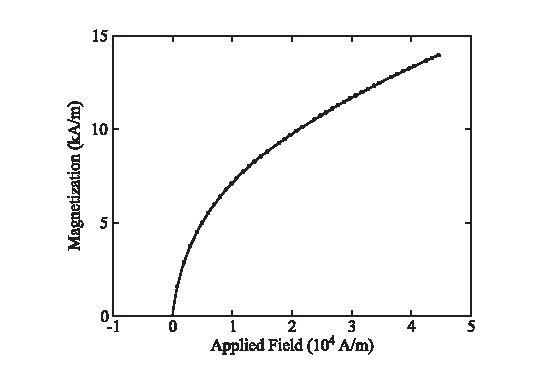
\includegraphics[scale=1]{Figs/figure.eps}
	\centering
	\caption{Magnetization as a function of applied field. (Note that ``Fig.'' is abbreviated and there is a period after the figure number followed by two spaces.) Font: \showfont}
	\label{fig:fig1}
\end{figure}

To better understand graphs, the definition of their axes should be done with words not letters, except when referring to waveforms and phase planes. The units should be between parentheses. For example, use the denomination ``Magnetization (A/m)'', instead of ``M (A/m)''.

Figures and tables should be positioned preferably in the beginning or the end of the column, avoiding putting them in the middle. Avoid tables and figures whose sizes exceed the size of the columns. The figures should preferentially be in black, with a white background, since the printed version of the journal is in black and white. Their lines should be thick, so the impression is readable.

\subsection{Abbreviations and Acronyms}
Abbreviations and acronyms must be defined the first time they are used in the text, e.g. ``... Pulse-Width Modulation (PWM)...''.

\subsection{Equations}
Number equations consecutively with equation numbers in parentheses flush with the right margin, as in (1). The equations should be written in a compact form, centered in the column. If a nomenclature section is not included in the beginning of the text, the quantities should be defined right after the equation, such as:
\begin{equation}
	\Delta I_{L}=I_{o}+\frac{\sqrt{3}}{2}\frac{V_{i}}{Z}
\end{equation} 
where: 

\symboldescription{$\Delta I_{L}$}{resonant inductor peak current;}
\symboldescription{$I_o$}{load current;}
\symboldescription{$V_i$}{source voltage;}
\symboldescription{$Z$}{characteristic impedance.}

\section{CONCLUSIONS}
This paper was fully written in accordance with the guidelines for submissions of papers in English.


\section*{ACKNOWLEDGEMENTS}
The authors thank John Doe for the collaboration of preparing this paper. This Project was financed by the CNPq (xxyyzz process).

% references section
\bibliographystyle{cobep-spec}
\balance
\bibliography{cobep-spec}



\end{document}
